\documentclass{article}
\usepackage{amsmath,amsthm,amssymb}
\usepackage{mathtext}
\usepackage[T1,T2A]{fontenc}
\usepackage[utf8]{inputenc}
\usepackage[russian]{babel}
\usepackage{graphicx}
\graphicspath{ {./} }

\begin{document}
    Описание решения\\\\
    Уравнение, описывающее систему, можно записать в виде:\\\\
    $\log_{10} Z = KT + C$, где $C = \frac{1024R_0}{R_C + R_0} - KT_0$\\\\
    Искомыми коэффициентами являются $C$ и $K$.\\\\
    Уравнения компонент неувязки:\\\\
    $r_i = T_{i}K + C - \log_{10}Z_i$\\\\
    Результат:\\\\
    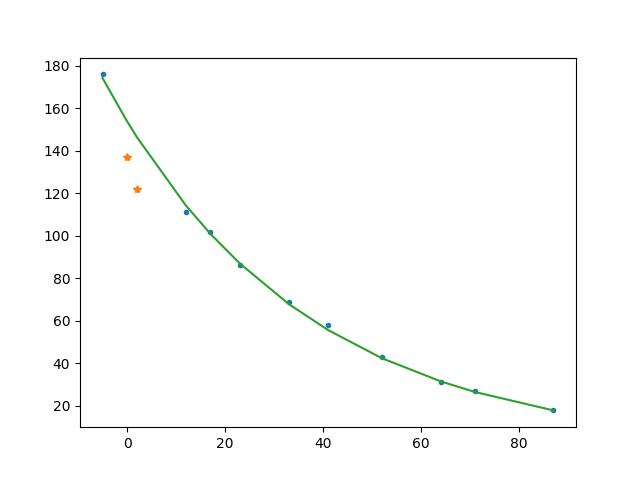
\includegraphics{graphic}
\end{document}